\subsection{Einfachste XOR-Verschlüsselung überhaupt}

Ich habe einmal eine Software gesehen, bei der alle Debugging-Ausgaben mit XOR mit dem Wert 3
verschlüsselt wurden. Mit anderen Worten, die beiden niedrigsten Bits aller Buchstaben wurden invertiert.

``Hello, world'' wurde zu ``Kfool/\#tlqog'':

\begin{lstlisting}
#!/usr/bin/python

msg="Hello, world!"

print "".join(map(lambda x: chr(ord(x)^3), msg))
\end{lstlisting}

Das ist eine ziemlich interessante Verschlüsselung (oder besser eine Verschleierung),
weil sie zwei wichtige Eigenschaften hat:
1) es ist eine einzige Funktion zum Verschlüsseln und entschlüsseln, sie muss nur wiederholt angewendet werden
2) die entstehenden Buchstaben befinden sich im druckbaren Bereich, also die ganze Zeichenkette kann ohne
Escape-Symbole im Code verwendet werden.

Die zweite Eigenschaft nutzt die Tatsache, dass alle druckbaren Zeichen in Reihen organisiert sind: 0x2x-0x7x,
und wenn die beiden niederwertigsten Bits invertiert werden, wird der Buchstabe um eine oder drei Stellen nach
links oder rechts \IT{verschoben}, aber niemals in eine andere Reihe:

\begin{figure}[H]
\centering
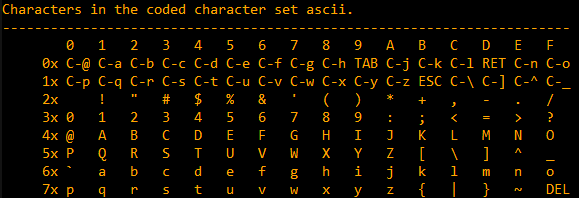
\includegraphics[width=0.7\textwidth]{ascii_clean.png}
\caption{7-Bit \ac{ASCII} Tabelle in Emacs}
\end{figure}

\dots mit dem Zeichen 0x7F als einziger Ausnahme.

Im Folgenden werden also beispielsweise die Zeichen A-Z \IT{verschlüsselt}:

\begin{lstlisting}
#!/usr/bin/python

msg="@ABCDEFGHIJKLMNO"

print "".join(map(lambda x: chr(ord(x)^3), msg))
\end{lstlisting}

Ergebnis:
% FIXME \verb  --  relevant comment for German?
\begin{lstlisting}
CBA@GFEDKJIHONML
\end{lstlisting}

Es sieht so aus als würden die Zeichen ``@'' und ``C'' sowie ``B'' und ``A'' vertauscht werden.

Hier ist noch ein interessantes Beispiel, in dem gezeigt wird, wie die Eigenschaften von XOR
ausgenutzt werden können: Exakt den gleichen Effekt, dass druckbare Zeichen auch druckbar bleiben,
kann man dadurch erzielen, dass irgendeine Kombination der niedrigsten vier Bits invertiert wird.
